\documentclass[border=10pt]{standalone}
\usepackage[svgnames]{xcolor}
\usepackage{amsmath}
\usepackage{pgfplots}
\pgfplotsset{compat=newest}
\usepackage[sfdefault]{FiraSans}
\usepackage{FiraMono}
\renewcommand*\familydefault{\sfdefault}
\begin{document}
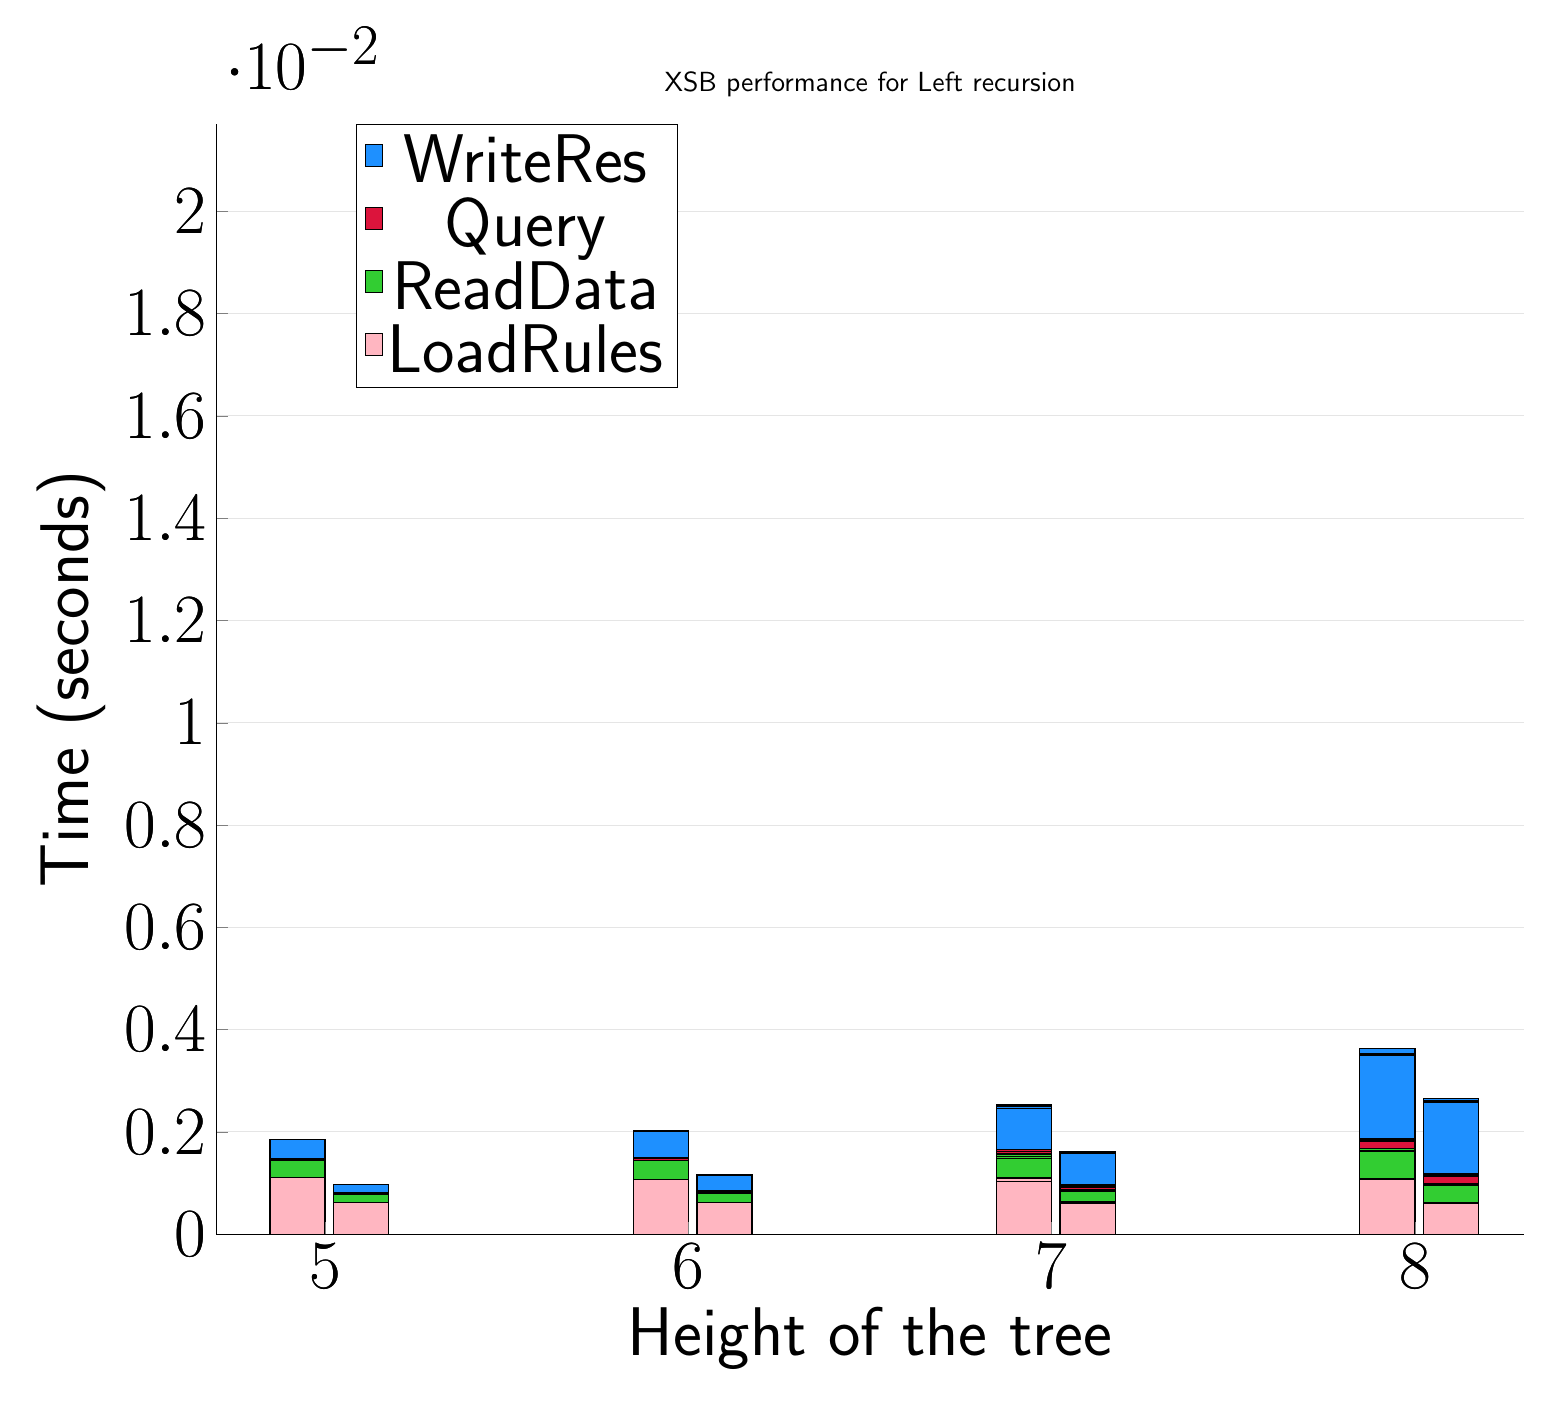
\begin{tikzpicture}
\begin{axis}[
   ybar stacked,
   title={XSB performance for Left recursion},
   bar shift=-10pt,
   width=1.5\textwidth,
   bar width=0.7cm,
   ymajorgrids, tick align=inside,
   major grid style={draw=gray!20},
   xtick=data,
   ymin=0, ymax=0.021717853546142578,
   axis x line*=bottom,
   axis y line*=left,
   enlarge x limits=0.1,
   legend style={
       at={(0.23, 1)},
       anchor=north,
       legend columns=1,
       font=\Huge,
   },
   ylabel={Time (seconds)},
   xlabel={Height of the tree},
   label style={font=\Huge},
   tick label style={font=\Huge},
]
\addlegendimage{fill=DodgerBlue, draw=black, line width=0.2pt}
\addlegendentry{WriteRes}
\addlegendimage{fill=Crimson, draw=black, line width=0.2pt}
\addlegendentry{Query}
\addlegendimage{fill=LimeGreen, draw=black, line width=0.2pt}
\addlegendentry{ReadData}
\addlegendimage{fill=LightPink, draw=black, line width=0.2pt}
\addlegendentry{LoadRules}
\addplot +[fill=LightPink, draw=black, line width=0.5pt] coordinates {
    (5, 0.0011033773422241219)
    (6, 0.001066088676452636)
    (7, 0.001031947135925293)
    (7, 0.0010866880416870101)
    (7, 0.0011097908020019532)
    (8, 0.0010694026947021492)
    (8, 0.001077818870544432)
    (8, 0.0010790586471557616)
};
\addplot +[fill=LimeGreen, draw=black, line width=0.5pt] coordinates {
    (5, 0.00034685134887695306)
    (6, 0.0003728866577148437)
    (7, 0.000449347496032715)
    (7, 0.0004359245300292968)
    (7, 0.0004486083984375)
    (8, 0.000553107261657715)
    (8, 0.0005602121353149414)
    (8, 0.0005972385406494141)
};
\addplot +[fill=Crimson, draw=black, line width=0.5pt] coordinates {
    (5, 2.9015541076660147e-05)
    (6, 4.820823669433595e-05)
    (7, 9.191036224365234e-05)
    (7, 9.038448333740235e-05)
    (7, 9.477138519287113e-05)
    (8, 0.0001963138580322267)
    (8, 0.000201702117919922)
    (8, 0.00019927024841308585)
};
\addplot +[fill=DodgerBlue, draw=black, line width=0.5pt] coordinates {
    (5, 0.0003746032714843752)
    (6, 0.0005347728729248049)
    (7, 0.0008869647979736328)
    (7, 0.0008854866027832028)
    (7, 0.0008698463439941406)
    (8, 0.0016892194747924814)
    (8, 0.001687407493591308)
    (8, 0.0017526149749755864)
};
\end{axis}
\begin{axis}[
   ybar stacked,
   bar shift=13pt,
   width=1.5\textwidth,
   bar width=0.7cm,
   ymajorgrids, tick align=inside,
   major grid style={draw=none},
   xtick=data,
   ymin=0, ymax=0.021717853546142578,
   axis x line*=none,
   axis y line*=none,
   enlarge x limits=0.1,
   label style={font=\Huge},
   tick label style={font=\Huge},
]
\addplot +[fill=LightPink, draw=black, line width=0.5pt] coordinates {
    (5, 0.000626)
    (6, 0.0006193)
    (7, 0.0005992000000000001)
    (7, 0.0006191000000000002)
    (7, 0.0006285999999999997)
    (8, 0.0006097)
    (8, 0.0006138999999999997)
    (8, 0.0006213000000000003)
};
\addplot +[fill=LimeGreen, draw=black, line width=0.5pt] coordinates {
    (5, 0.00015739999999999998)
    (6, 0.00018460000000000029)
    (7, 0.0002425000000000001)
    (7, 0.00023899999999999993)
    (7, 0.00024559999999999984)
    (8, 0.00034490000000000004)
    (8, 0.00035350000000000014)
    (8, 0.00036599999999999946)
};
\addplot +[fill=Crimson, draw=black, line width=0.5pt] coordinates {
    (5, 2.319999999999961e-05)
    (6, 4.119999999999993e-05)
    (7, 8.46999999999997e-05)
    (7, 8.470000000000022e-05)
    (7, 8.800000000000035e-05)
    (8, 0.0001861000000000006)
    (8, 0.00019009999999999974)
    (8, 0.0001899000000000008)
};
\addplot +[fill=DodgerBlue, draw=black, line width=0.5pt] coordinates {
    (5, 0.00015960000000000022)
    (6, 0.0003096000000000005)
    (7, 0.000655)
    (7, 0.0006519999999999996)
    (7, 0.0006555999999999995)
    (8, 0.0014469999999999995)
    (8, 0.0014550000000000003)
    (8, 0.0014720999999999992)
};
\end{axis}
\end{tikzpicture}

\end{document}
